\documentclass{article}
\usepackage{physics}
\usepackage{graphicx}
\usepackage{float}
\usepackage{amsmath}
\usepackage{mathtools}
% Please add the following required packages to your document preamble:
\usepackage[table,xcdraw]{xcolor}
% If you use beamer only pass "xcolor=table" option, i.e. \documentclass[xcolor=table]{beamer}
\usepackage[normalem]{ulem}
\useunder{\uline}{\ul}{}

\author{Philip Renkert}
\date{6/15/2021}

\newcommand{\defeq}{\vcentcolon=}

\begin{document} 
	\section*{Coordinate System and Attitude Representation}
	Two coordinate frames are employed to describe the state of the quadrotor:
	\begin{itemize}
		\item Earth Coordinate Frame ($o_e x_e y_e z_e$): The initial position of the quadrotor defines the origin $o_e$ of this coordinate frame.  The $0_e x_e$ axis points in a given fixed direction in the horizontal plane, the $o_e z_e$ axis points downward toward the earth's center, and the $o_e y_e$ axis is determined according to the right hand rule.  
		\item Body Coordinate Frame ($o_b x_b y_b z_b$): This coordinate frame is attached to the quadrotor, and the quadrotor's center of gravity is chosen as its origin $o_b$. The $o_bx_b$ axis points in the nose direction as indicated in Figure~\ref{fig:body_frame}.  The $o_b z_b$ axis points downward perpendicular to the $o_b x_b$ axis.  The $o_b y_b$ axis is determined from the right hand rule.  
	\end{itemize}
	
	The relationship between the two coordinate systems is depicted in Figure~\ref{fig:coord_sys}.  A left superscript is used to indicate the frame to which a vector is relative, i.e. ${}^e \mathbf{x}$ is a vector relative to the earth frame and ${}^b \mathbf{x}$ is a vector relative to the body frame.  We must also define a standard basis with unit vectors $\mathbf{e}_1 \defeq \left[1,0,0\right]^\top$, $\mathbf{e}_2 \defeq \left[0,1,0\right]^\top$, and $\mathbf{e}_3 \defeq \left[0,0,1\right]^\top$.  In the earth frame, the axes $o_e x_e$, $o_e y_e$, and $o_e z_e$ are expressed with $\mathbf{e}_1$, $\mathbf{e}_2$, and $\mathbf{e}_3$ respectively. Body unit vectors $\mathbf{b}_1 \defeq o_b x_b$, $\mathbf{b}_2 \defeq o_b y_b$, and $\mathbf{b}_3 \defeq o_b z_b$ can be expressed relative to the body frame as ${}^b \mathbf{b}_i = \mathbf{e}_i$ and relative to the earth frame as ${}^e \mathbf{b}_i$ for all $i \in \left\{1,2,3\right\}$. 
	
	\begin{figure}[H]
		\centering
		\begin{minipage}[t]{0.48\linewidth}
			\centering
			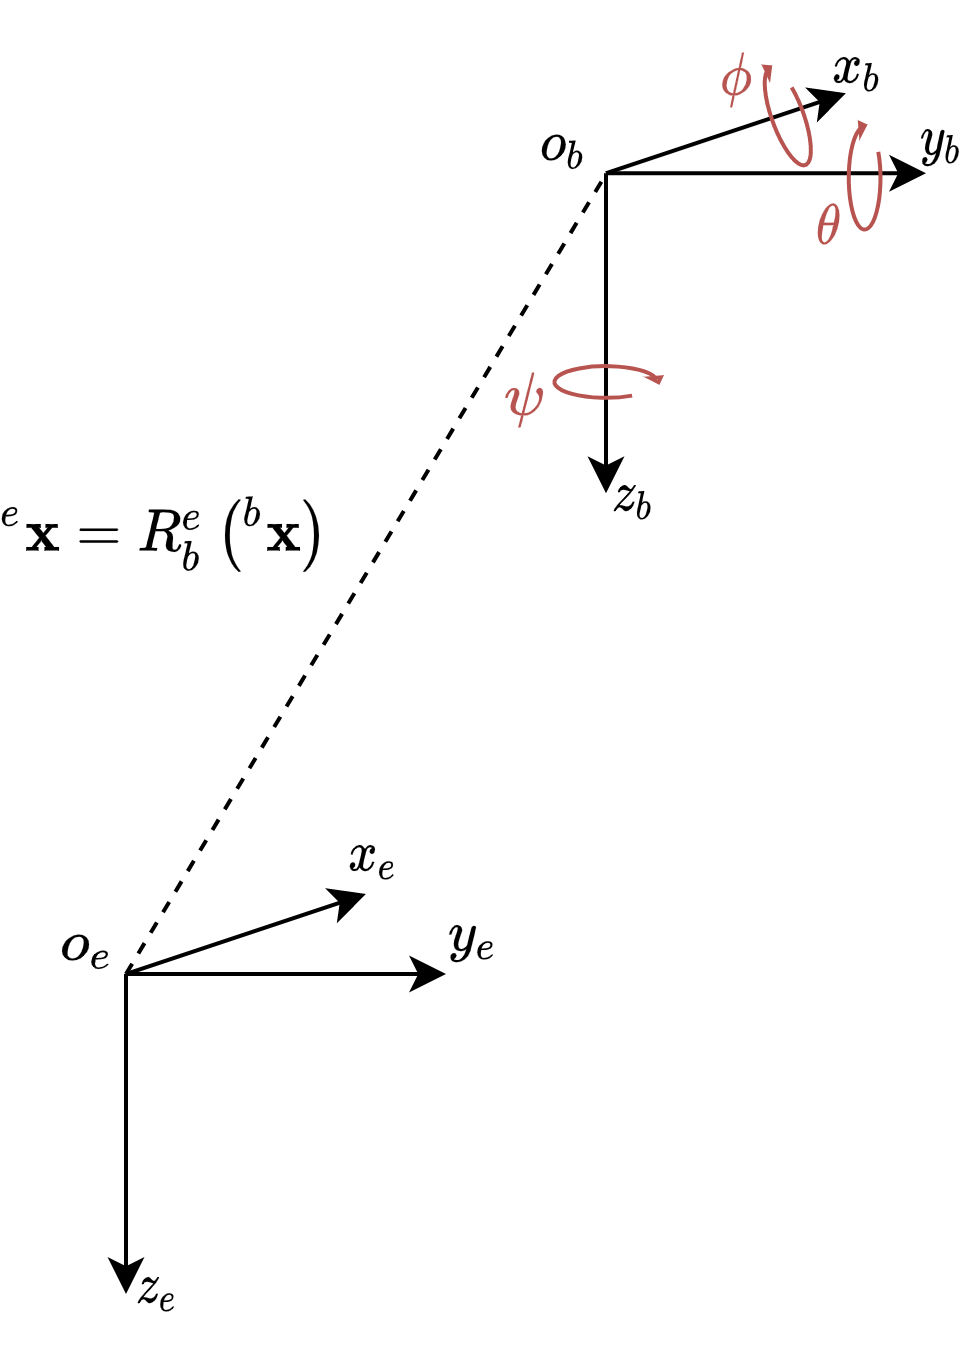
\includegraphics[height = \linewidth]{3DCoordinateSystems.png}
			\caption{Coordinate system representation}
			\label{fig:coord_sys}
		\end{minipage}
		\begin{minipage}[t]{0.48\linewidth}
			\centering
			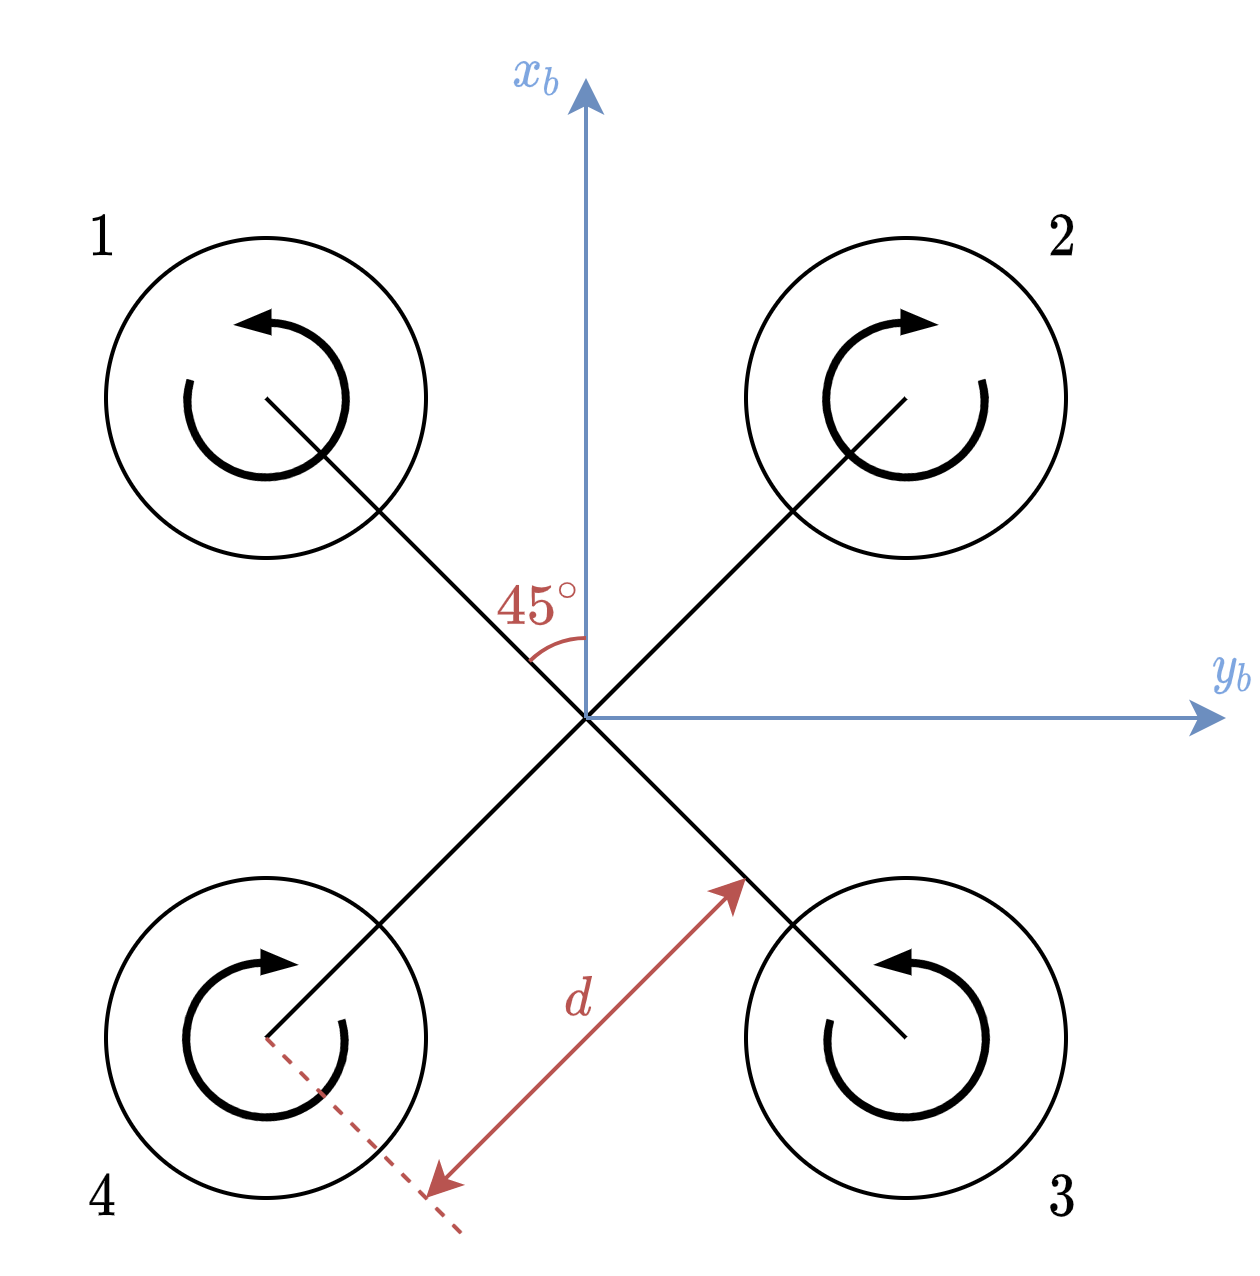
\includegraphics[height = \linewidth]{BodyFrameDiagram.png}
			\caption{Body frame coordinate system, top-down view}
			\label{fig:body_frame}
		\end{minipage}
	\end{figure}

	The aircraft's attitude will be expressed with Euler angles $\psi$ (yaw angle), $\theta$ (pitch angle), and $\phi$ (roll angle).  The body orientation is achieved by three successive rotations about the $z$, $y$, and $x$ axes around a fixed point. Let the frame resulting from the first elemental rotation be $k$ with unit vectors $\mathbf{k}_i$ and that of the second elemental rotation be $n$ with unit vectors $\mathbf{n}_i$. Frame $k$ is achieved by a yaw rotation about the $\mathbf{e}_3$ axis by $\psi$. Frame $n$ is achieved by a pitch rotation about the $\mathbf{k}_2$ axis by $\theta$.  The final body frame is achieved by a roll rotation about the $\mathbf{n}_1$ axis by $\phi$.  The combined rotation can be expressed as the product of three rotation matrices.  Denote a rotation matrix that performs a change of basis from frame $a$ to frame $b$ (rotation of frame $a$ relative to fixed frame $b$) as $\mathbf{R}_a^b$. The elemental rotation matrices are,
	\begin{align}
		\begin{split}
		\mathbf{R}_z(\psi) &= 
		\left(
		\begin{array}{ccc}
			\cos (\psi ) & \sin (\psi ) & 0 \\
			-\sin (\psi ) & \cos (\psi ) & 0 \\
			0 & 0 & 1 \\
		\end{array}
		\right)
		\\
		\mathbf{R}_y(\theta) &= 
		\left(
		\begin{array}{ccc}
			\cos (\theta ) & 0 & -\sin (\theta ) \\
			0 & 1 & 0 \\
			\sin (\theta ) & 0 & \cos (\theta ) \\
		\end{array}
		\right)\\
		\mathbf{R}_x(\phi) &= 
		\left(
		\begin{array}{ccc}
			1 & 0 & 0 \\	
			0 & \cos (\phi ) & \sin (\phi ) \\
			0 & -\sin (\phi ) & \cos (\phi ) \\
		\end{array}
		\right)
		\end{split}
	\end{align}
	The combined rotation matrix that transforms a vector $\mathbf{x}$ expressed in the earth frame ${}^e \mathbf{x}$ into a vector expressed in the body frame ${}^b \mathbf{x}$ is then,
	\begin{equation}
		{}^b \mathbf{x} = \mathbf{R}_n^b \mathbf{R}_k^n \mathbf{R}_e^k\left( {}^e \mathbf{x}\right) =\mathbf{R}_e^b\left( {}^e \mathbf{x}\right)
	\end{equation}
	Where $\mathbf{R}_n^b = R_x(\phi)$, $\mathbf{R}_k^n = R_y(\theta)$, and $\mathbf{R}_e^k = R_z(\psi)$.  Performing the matrix multiplication gives,
	\begin{equation}
		\mathbf{R}_e^b = \left(
		\begin{array}{ccc}
			\text{c} (\theta ) \text{c} (\psi ) & \text{c} (\theta ) \text{s}  (\psi ) & -\text{s}  (\theta ) \\
			\text{s}  (\theta ) \text{c} (\psi ) \text{s}  (\phi )-\text{s}  (\psi ) \text{c} (\phi ) & \text{s}  (\theta ) \text{s}  (\psi ) \text{s}  (\phi )+\text{c} (\psi ) \text{c} (\phi ) & \text{c} (\theta ) \text{s}  (\phi ) \\
			\text{s}  (\theta ) \text{c} (\psi ) \text{c} (\phi )+\text{s}  (\psi ) \text{s}  (\phi ) & \text{s}  (\theta ) \text{s}  (\psi ) \text{c} (\phi )-\text{c} (\psi ) \text{s}  (\phi ) & \text{c} (\theta ) \text{c} (\phi ) \\
		\end{array}
		\right)
	\end{equation}
	Where $\text{c}()$ is an abbreviation of $\cos()$ and $\text{s}()$ is n abbreviation of $\sin()$. 
	\section*{Rigid-body Kinematic Model}
		In order to analyze the kinetics of the aircraft, we must first understand the relationship between the angular velocity of the body ${}^b\mathbf{\omega} = \left[p,q, r\right]^\top$ and the  attitude rate $\dot{\mathbf{\Theta}} = \left[\dot{\phi}, \dot{\theta}, \dot{\psi}\right]^\top$. To do so, we'll the theorem involving the time derivative of rotation matrices from Zhao in \cite{zhaoTimeDerivativeRotation2016} given in Equation~\ref{eq:rot_matrix_derivative}.  
		\begin{equation}
			\dv{}{t}{\mathbf{R}_b^e} = \mathbf{R}_b^e \left[{}^b \mathbf{\omega}\right]_{\cross}
			\label{eq:rot_matrix_derivative}
		\end{equation}
		Where $\left[\cdot\right]_{\cross}$ is the skew symmetric operator used to convert a cross product of two vectors into a matrix-vector product.  Rearranging \ref{eq:rot_matrix_derivative} gives,
		\begin{equation}
			\left[{}^b \mathbf{\omega}\right]_{\cross} = {\mathbf{R}_b^e}^\top \dv{}{t}{\mathbf{R}_b^e} = {\mathbf{R}_e^b} \dv{}{t}{\mathbf{R}_b^e}
		\end{equation}
		We'll employ the chain rule to expand the derivative
		\begin{equation}
			\left[{}^b \mathbf{\omega}\right]_{\cross} = {\mathbf{R}_b^e}^\top \dv{}{t}{\mathbf{R}_b^e} = {\mathbf{R}_e^b} \left(\dv{\mathbf{R}_b^e}{\phi}\dot{\phi} + \dv{\mathbf{R}_b^e}{\theta}\dot{\theta} + \dv{\mathbf{R}_b^e}{\psi}\dot{\psi}\right)
		\end{equation}
		We'll simplify the expression to achieve a linear relationship between ${}^b \mathbf{\omega}$ and $\dot{\mathbf{\Theta}}$.   
		\begin{equation}
			{}^b\mathbf{\omega} = 
			\left(
			\begin{array}{ccc}
				1 & 0 & -\sin(\theta) \\	
				0 & \cos (\phi ) & \cos(\theta)\sin (\phi ) \\
				0 & -\sin (\phi ) & \cos(\theta)\cos (\phi ) \\
			\end{array}
			\right) \dot{\mathbf{\Theta}} =\vcentcolon \mathbf{W}^{-1} \dot{\mathbf{\Theta}}
		\end{equation}
		Taking the inverse,
		\begin{equation}
			\dot{\mathbf{\Theta}} =\mathbf{W}\cdot{}^b\mathbf{\omega} = \left(
			\begin{array}{ccc}
				1 & \tan (\theta ) \sin (\phi ) & \tan (\theta ) \cos (\phi ) \\
				0 & \cos (\phi ) & -\sin (\phi ) \\
				0 & \sin{\phi}/\cos{\theta} & \cos (\phi ) / \cos (\theta ) \\
			\end{array}
			\right)
			{}^b\mathbf{\omega}
		\end{equation}
		Our kinematic equations for the quadrotor body can finally be written.  Let $\mathbf{p}$ represent the position of the quadrotor's center of gravity (i.e. $o_b$)  and $\mathbf{v}$ represent the linear velocity.  
		\begin{align}
			\begin{split}
				{}^e \dot{\mathbf{p}} &= {}^e \mathbf{v} \\
				\dot{\mathbf{\Theta}} &= \mathbf{W} \cdot {}^b\mathbf{\omega}
			\end{split}
			\label{eq:kinematic_equations}
		\end{align}
	
		Note: We can also work directly with rotation matrices instead of Euler angles if it makes for a better starting point.  
	\section*{Rigid-body Dynamic Model}
	\textit{Position Dynamic Model}:
	With level propellers producing thrust parallel to $\mathbf{b}_3$, the position dynamics are described by Equation~\ref{eq:pos_dyn_1}:
	\begin{equation}
		{}^e\dot{\mathbf{v}} = g \mathbf{e}_3 - \frac{f}{m}{}^e\mathbf{b}_3
		\label{eq:pos_dyn_1}
	\end{equation}
	where $g$ is the gravitational acceleration, $f$ is the combined thrust produced by the four propellers calculated in the control effectiveness model, and $m$ is the mass of the aircraft.  We can then use the rotation matrix $\mathbf{R}_b^e$ to find ${}^e\mathbf{b}_3$.  Since
	\begin{equation}
		{}^e \mathbf{v} =\mathbf{R}_b^e \cdot {}^b\mathbf{v}
		\label{eq:pos_dyn_2}
	\end{equation}
	we have,
	\begin{equation}
		{}^e\dot{\mathbf{v}} = g \mathbf{e}_3 + \frac{1}{m}\mathbf{R}_b^e\cdot{}^b\mathbf{f}_3
		\label{eq:pos_dyn_final}
	\end{equation}
	where ${}^b\mathbf{f}_3 \defeq -f\mathbf{e}_3$.
	\newline \newline \textit{Attitude Dynamic Model}:  We'll start with Euler's equation describing the rotation of a rigid body \cite{ClassicalDynamicsParticles1965}: 
	\begin{equation}
		\mathbf{J} \cdot {}^b\dot{\mathbf{\omega}} + {}^b\mathbf{\omega} \cross \mathbf{J}\cdot{}^b\mathbf{\omega}= \mathbf{M}
		\label{eq:euler_eqn}
	\end{equation}
	Where $\mathbf{J}$ is the inertia tensor relative to the body frame, ${}^b\mathbf{\omega}$ is the angular velocity defined above, and $\mathbf{M}$ is the sum of the moments acting on the craft in the body frame.  For a simple quadrotor model, $\mathbf{M}$ comes from two primary sources: moments generated by the propellers $\mathbf{\tau} = \left[\tau_x, \tau_y, \tau_z\right]^\top$ and the gyroscopic torques associated with the rotors $\mathbf{G}_a = \left[G_{a,x}, G_{a,y}, G_{a,z}\right]$.  $\mathbf{\tau}$ is calculated in the control effectiveness model in the next section, as each of the moments is simply related to the square the rotor speed.
	\begin{equation}
		\mathbf{M} = \mathbf{\tau} + \mathbf{G}_a
	\end{equation}  
	The gyroscopic torque of the $k_{th}$ rotor is found again by looking at the torque acting on the rotor in the rotating body frame,
	\begin{equation}
		\mathbf{G}_{a,k} = - \left(\dv{}{t}\left({}^b \mathbf{L}_k\right) + {}^b\mathbf{\omega} \cross {}^b \mathbf{L}_k\right)
		\label{eq:gyro_torque}
	\end{equation}
	Where ${}^b \mathbf{L}_k$ is the angular momentum contributed by rotor $k$ relative to the body frame. The quantity in parenthesis in the right-hand side of Equation~\ref{eq:gyro_torque} represents the external moments in the body frame acting on rotor $k$ given the body's angular velocity ${}^b\mathbf{\omega}$.  $\mathbf{G}_{a,k}$ is therefore the torque exerted on the body by rotor $k$. ${}^b \mathbf{L}_k$ is simply the rotor's inertia about its central axis $J_r$ times its angular velocity vector in the body frame ${}^b \mathbf{\omega}_k$.
	\begin{equation}
		{}^b \mathbf{L}_k = J_r \cdot {}^b \mathbf{\omega}_k = J_r\left(-1^k\right) \tilde{\omega}_k \mathbf{e}_3
		\label{eq:rotor_momentum}
	\end{equation}
	where $\tilde{\omega}_k$ is the unsigned angular speed of rotor $k$.  Note that $\dv{}{t}\left({}^b \mathbf{L}_k\right)$ is zero if we assume that $\tilde{\omega}_k$ is constant.  This allows us to write,
	\begin{equation}
		\mathbf{G}_{a,k} = - \left({}^b\mathbf{\omega} \cross {}^b \mathbf{L}_k\right) = {}^b \mathbf{L}_k \cross {}^b\mathbf{\omega}
		\label{eq:rotor_gyro_torque_simple}
	\end{equation}
	Substituting \ref{eq:rotor_momentum} into \ref{eq:rotor_gyro_torque_simple} gives,
	\begin{equation}
		\mathbf{G}_{a,k} = J_r\left(-1^k\right) \tilde{\omega}_k \mathbf{e}_3 \cross {}^b\mathbf{\omega}
	\end{equation}
	The total gyroscopic torque is then,
	\begin{equation}
		\mathbf{G}_a = \sum_{k=1}^{N_r}{\mathbf{G}_{a,k}} = J_r\left(\mathbf{e}_3\cross{}^b\mathbf{\omega}\right)\sum_{k=1}^{N_r}{\left(-1^k\right) \tilde{\omega}_k} = J_r\left(\sum_{k=1}^{N_r}{\left(-1^k\right) \tilde{\omega}_k}\right)  \left[\mathbf{e}_3\right]_{\cross}{}^b\mathbf{\omega}
	\end{equation}
	It remains to calculate the inertia tensor. 
	\section*{Parametric Inertia Tensor}
		A dynamic model for design optimization must be parametrized by the design variables.  Because the inertial properties of the quadrotor will change depending on the motor, propeller, and battery design, the inertial tensor must be expressed as a function of these elements.  Most examples of quadrotor dynamics and simulation in the literature determine the inertia tensor  by 1) conducting physical experiments such as a bifilar pendulum \cite{quanIntroductionMulticopterDesign2017} or 2) building a detailed CAD model of the system.  Though accurate, neither of these approaches can account for changes in the physical design and therefore aren't compatible with design optimization.  
		\par We can, however, use a hybrid numerical and analytical approach.  First, the inertial tensor $\mathbf{J}_{f}$ of the 'fixed' system (i.e. excluding the battery, motors, and propellers) is calculated via CAD or physical experiments. Then, the inertia matrix for each of the optimization components $\mathbf{J}_{c,i}^{\prime}$ is calculated analytically about the component's center of mass. Then, the generalized parallel axis theorem is used to calculate each components' inertia about the system's center of mass $\mathbf{J}_{c,i}$.  The formula for the generalized parallel axis theorem is given in \cite{ParallelAxisTheorem2021} as Equation~\ref{eq:parallel_axis_theorem}:
		\begin{equation}
			\mathbf{J}_{c,i} = \mathbf{J}_{c,i}^{\prime} + m_{c,i}\left(\norm{\mathbf{r}_{c,i}}^2 I_3 - \mathbf{r}_{c,i} \otimes \mathbf{r}_{c,i} \right)
			\label{eq:parallel_axis_theorem}
		\end{equation}
		Finally, the system inertia tensor $\mathbf{J}$ is found by summing each individual inertia tensor:
		\begin{equation}
		\mathbf{J} = \mathbf{J}_f + \sum_{c,i}{\mathbf{J}_{c,i}}
		\label{eq:system_inertia_tensor}
		\end{equation}
		
		For now, we'll simplify Equations~\ref{eq:parallel_axis_theorem} and~\ref{eq:system_inertia_tensor} by assuming the motor and propeller are point masses at the end of each arm and the battery is a point mass at the system's center of gravity.  Though these assumptions make for a very rough approximation, they should capture the general trend of how design changes impact the real system's inertial properties.  Applying Equation~\ref{eq:parallel_axis_theorem} to the rotors $r$ gives
		\begin{equation}
			\mathbf{J}_{r,k} = \left(m_{\text{prop}} + m_{\text{motor}}\right) \left(\norm{\mathbf{r}_{r,k}}^2 I_3 - \mathbf{r}_{r,k} \otimes \mathbf{r}_{r,k} \right)
			\label{eq:parallel_axis_theorem_rotor}
		\end{equation}
		The displacement from the system's center of mass to the rotors' center of mass $\mathbf{r}_{r,k}$ is approximately
		\begin{align}
		\begin{split}
			\mathbf{r}_{r,1} &= d\frac{\sqrt{2}}{2}\begin{bmatrix} -1 & 1 & 0\end{bmatrix}^\top \\
			\mathbf{r}_{r,2} &= d\frac{\sqrt{2}}{2}\begin{bmatrix} 1 & 1 & 0\end{bmatrix}^\top \\
			\mathbf{r}_{r,3} &= d\frac{\sqrt{2}}{2}\begin{bmatrix} 1 & -1 & 0\end{bmatrix}^\top \\
			\mathbf{r}_{r,4} &= d\frac{\sqrt{2}}{2}\begin{bmatrix} -1 & -1 & 0\end{bmatrix}^\top
		\end{split}
		\end{align}
		
		Where $d$ is the distance from the system's center of mass to that of the rotor as shown in Figure~\ref{fig:body_frame}.  
		Applying Equation~\ref{eq:parallel_axis_theorem_rotor} and summing over all four rotors gives the moments of inertia contributed by the rotors.
		\begin{equation}
			\mathbf{J}_r = \sum_{k=1}^{4}{\mathbf{J}_{r,k}} = \left(m_{\text{prop}} + m_{\text{motor}}\right)d^2
			\begin{bmatrix}
				2 & 0 & 0 \\ 0 & 2 & 0 \\ 0 & 0 & 4
			\end{bmatrix}
		\end{equation}
		By assuming the battery is a point mass at the system's center of mass, the battery's inertia $\mathbf{J}_b = 0$. Therefore, we can write a simplified version of the system's inertia tensor in Equation~\ref{eq:system_inertia_tensor} as,
		\begin{equation}
			\mathbf{J} = \mathbf{J}_f + \mathbf{J}_r
		\end{equation}
		I'm currently working on a CAD model to calculate $\mathbf{J}_f$, though I anticipate its contribution will be small relative to that of $\mathbf{J}_r$.  
		
		
	\section*{Combined Dynamic Model}
		Equations~\ref{eq:kinematic_equations},~\ref{eq:pos_dyn_final}, and~\ref{eq:euler_eqn} can be combined to give a nonlinear model for the system's dynamics:
		\begin{equation}
			\begin{bmatrix} {}^e \dot{\mathbf{p}} \\ {}^e \dot{\mathbf{v}} \\ \dot{\mathbf{\Theta}} \\ {}^b\dot{\mathbf{\omega}} \end{bmatrix}
			 = 
			 \begin{bmatrix}
			 	{}^e \mathbf{v} \\
			 	g \mathbf{e}_3 + \frac{1}{m}\mathbf{R}_b^e\cdot{}^b\mathbf{f}_3 \\
			 	\mathbf{W} \cdot {}^b\mathbf{\omega} \\
			 	\mathbf{J}^{-1}\left(-{}^b\mathbf{\omega} \cross \mathbf{J}\cdot{}^b\mathbf{\omega} +  \mathbf{\tau} + \mathbf{G}_a\right)
			 \end{bmatrix}
		\end{equation}
		Recall that the inputs to the dynamic model are $f$ and $\mathbf{\tau}$.  
	\section*{Control Effectiveness Model (Thrusts/Torques)}
		It remains to calculate $f$ and $\mathbf{\tau}$ as a function of the propeller speeds.  Let $C_T = k_T \rho D^4$ be the lumped thrust coefficient and $C_Q = k_Q \rho D^5$ be the lumped drag coefficient such that, for each propeller $k$, the thrust $T_k$ and torque $Q_k$ produced by each propeller is
		\begin{align}
			\begin{split}
				T_k &= C_T \tilde{\omega}_k^2 \\
				Q_k &= C_Q \tilde{\omega}_k^2
			\end{split}
		\end{align}
		The combined thrust $f$ is simply the sum of the thrusts generated by each propeller
		\begin{equation}
			f = C_T \sum_{k=1}^{N_r}{ \tilde{\omega}_k^2}
			\label{eq:combined_thrust}
		\end{equation}
		Similarly, the combined moment about the ${}^b \mathbf{b}_3$ axis $\tau_z$ is the sum of the torques generated by each propeller.  
		\begin{equation}
			\tau_z = C_Q \sum_{k=1}^{N_r}{\left(-1\right)^{k-1} \tilde{\omega}_k^2}
		\end{equation}
		Where the alternating sign comes from the rotors' alternating directions.  To calculate $\tau_x$ and $\tau_y$, note from Figure~\ref{fig:body_frame} that the moment arm of each propeller about the ${}^b \mathbf{b}_1$ and ${}^b \mathbf{b}_2$ axis is,
		\begin{equation}
			l = d \sin{45^\circ} = \frac{\sqrt{2}}{2}d
		\end{equation}
		Therefore,
		\begin{align}
			\begin{split}
				\tau_x &= lC_T\left(\tilde{\omega}_1^2 - \tilde{\omega}_2^2 - \tilde{\omega}_3^2 + \tilde{\omega}_4^2\right)\\
				\tau_y &=  lC_T\left(\tilde{\omega}_1^2 + \tilde{\omega}_2^2 - \tilde{\omega}_3^2 - \tilde{\omega}_4^2\right)
			\end{split}
			\label{eq:horizontal_torques}
		\end{align}
		Equations~\ref{eq:combined_thrust} - \ref{eq:horizontal_torques} can be written in matrix form as,
		\begin{equation}
			\begin{bmatrix}f \\ \tau_x \\ \tau_y \\ \tau_z \end{bmatrix} = 
			\begin{bmatrix}
				C_T & C_T & C_T & C_T \\ 
				lC_T & -lC_T & -lC_T & lC_T \\
				lC_T & lC_T & -lC_T & -lC_T \\
				C_Q & -C_Q & C_Q & -C_Q \\ 
			\end{bmatrix}
			\begin{bmatrix} \tilde{\omega}_1^2 \\ \tilde{\omega}_2^2 \\ \tilde{\omega}_3^2 \\ \tilde{\omega}_4^2 \end{bmatrix}
		\end{equation}
	
	\newpage
	\bibliography{ARGReferences}
	\bibliographystyle{plain}
\end{document}
